%!TEX root = CooperBarba-orientation.tex

We are aiming to investigate the orientation of proteins near self-assembled monolayers (\sam), specifically for biosensing applications. In the framework of the implicit-solvent model, we can represent the \sam\ as a surface charge density, and use Equation \eqref{eq:matrix_dphi} to compute the electrostatic potential. 
According to the Boltzmann distribution, the probability of finding the system in micro-state $\lambda$ depends on the total free energy, $F_\text{total}$, as follows:
%
\begin{equation} \label{eq:prob}
P(\lambda) = \frac{\int_{\lambda} \exp \left(-\frac{F_\text{total}}{k_B T} \right) \text{d} \lambda}{\int_{\Lambda} \exp \left(-\frac{F_\text{total}}{k_B T} \right) \text{d} \Lambda},
\end{equation} 

\noindent where $\Lambda$ is the ensemble of all micro-states, $k_B$ is the Boltzmann constant and $T$ the temperature. To obtain a probability distribution, we assume that electrostatic effects are dominant and used Equation \eqref{eq:prob}, sampling $F_\text{total}$ for different orientations. We defined the orientation using the angle between the dipole moment and surface normal vectors as a reference (tilt angle), varying from 0$^\circ$ to 180$^\circ$. For each tilt angle, we rotated the protein about the dipole moment vector by 360$^\circ$ to examine all possible orientations. This process is sketched in Figure \ref{fig:1pgb_orientation}.

In this case, micro-states are defined by the tilt ($\alpha_{\text{tilt}}$) and rotational ($\alpha_{\text{rot}}$) angles, and we rewrite the integral in the numerator of Equation \eqref{eq:prob} as:
%
\begin{equation} \label{eq:prob_angle}
\int_{\lambda} \exp \left(-\frac{F_\text{total}}{k_B T} \right) \text{d} \lambda = \int \int \exp \left(-\frac{F_\text{total}}{k_B T} \right) \text{d} \alpha_{\text{rot}} \text{d} \alpha_{\text{tilt}},
\end{equation}

\noindent where micro-state $\lambda$ is a range of angles $\alpha_{\text{rot}}$ and $\alpha_{\text{tilt}}$. 
In biosensors, the ligand is adsorbed on the surface (usually covalently), hence we are interested on the orientation of the molecule very close to the surface, and don't consider configurations away from it.  


\begin{figure}%[h] 
   \centering
   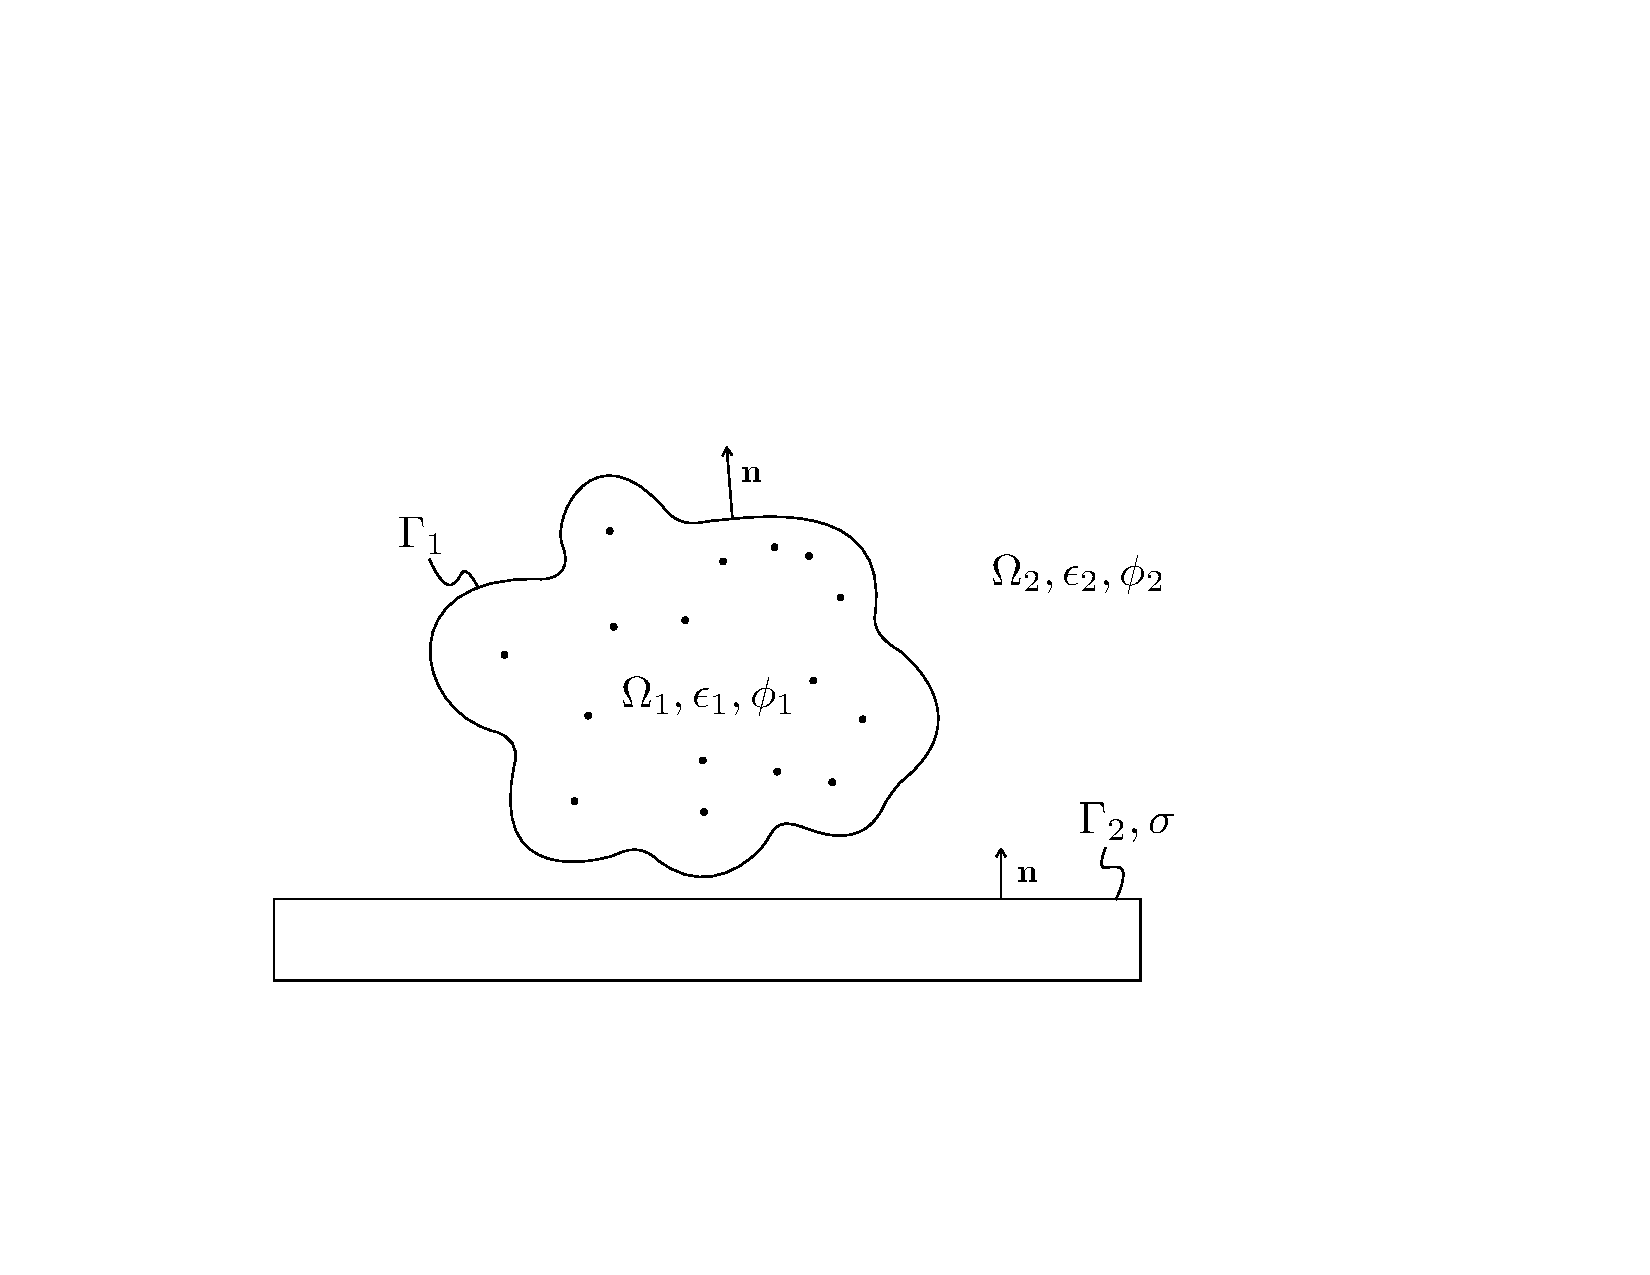
\includegraphics[width=0.5\textwidth]{Figure2.pdf}
   \caption{Setup of the problem for our orientation-sampling studies.}
   \label{fig:1pgb_orientation}
\end{figure}

\subsection{Structure preparation}

To assess the adequacy of the implicit-solvent model for investigating protein-surface interactions, we studied the orientation of protein \gb mutant near a charged surface, since there are results available in the literature that we could compare to: both experimental observations \cite{BaioWeidnerBaughGambleStaytonCastner2012} and simulations using a combined Monte Carlo and molecular dynamics approach.\cite{LiuLiaoZhou2013} Figure \ref{fig:1pgb} shows the structure of protein \gb (\pdb code {\small 1PGB}), to which we applied mutations {\small E19Q}, {\small D22N}, {\small D46N} and {\small D47N} to obtain the {\small D4$^\prime$} mutant, using the \textsl{SwissPdb Viewer} software.\cite{GuexPeitsch1997}
We then studied the orientation of antibody immunoglobulin G iso-type \ig 2a (\pdb code {\small 1IGT}), a widely used protein in biosensors, whose structure is shown in Figure \ref{fig:1igt}. This is a more interesting case from the point of view of our application, yet it is more difficult to study with molecular simulation due to its size.
In both cases, the vector orientation of the dipole moment (used as reference for the tilt and orientation angles) was obtained using the location of the point charges at the locations of the atoms.

\begin{figure}%[h] 
   \centering
   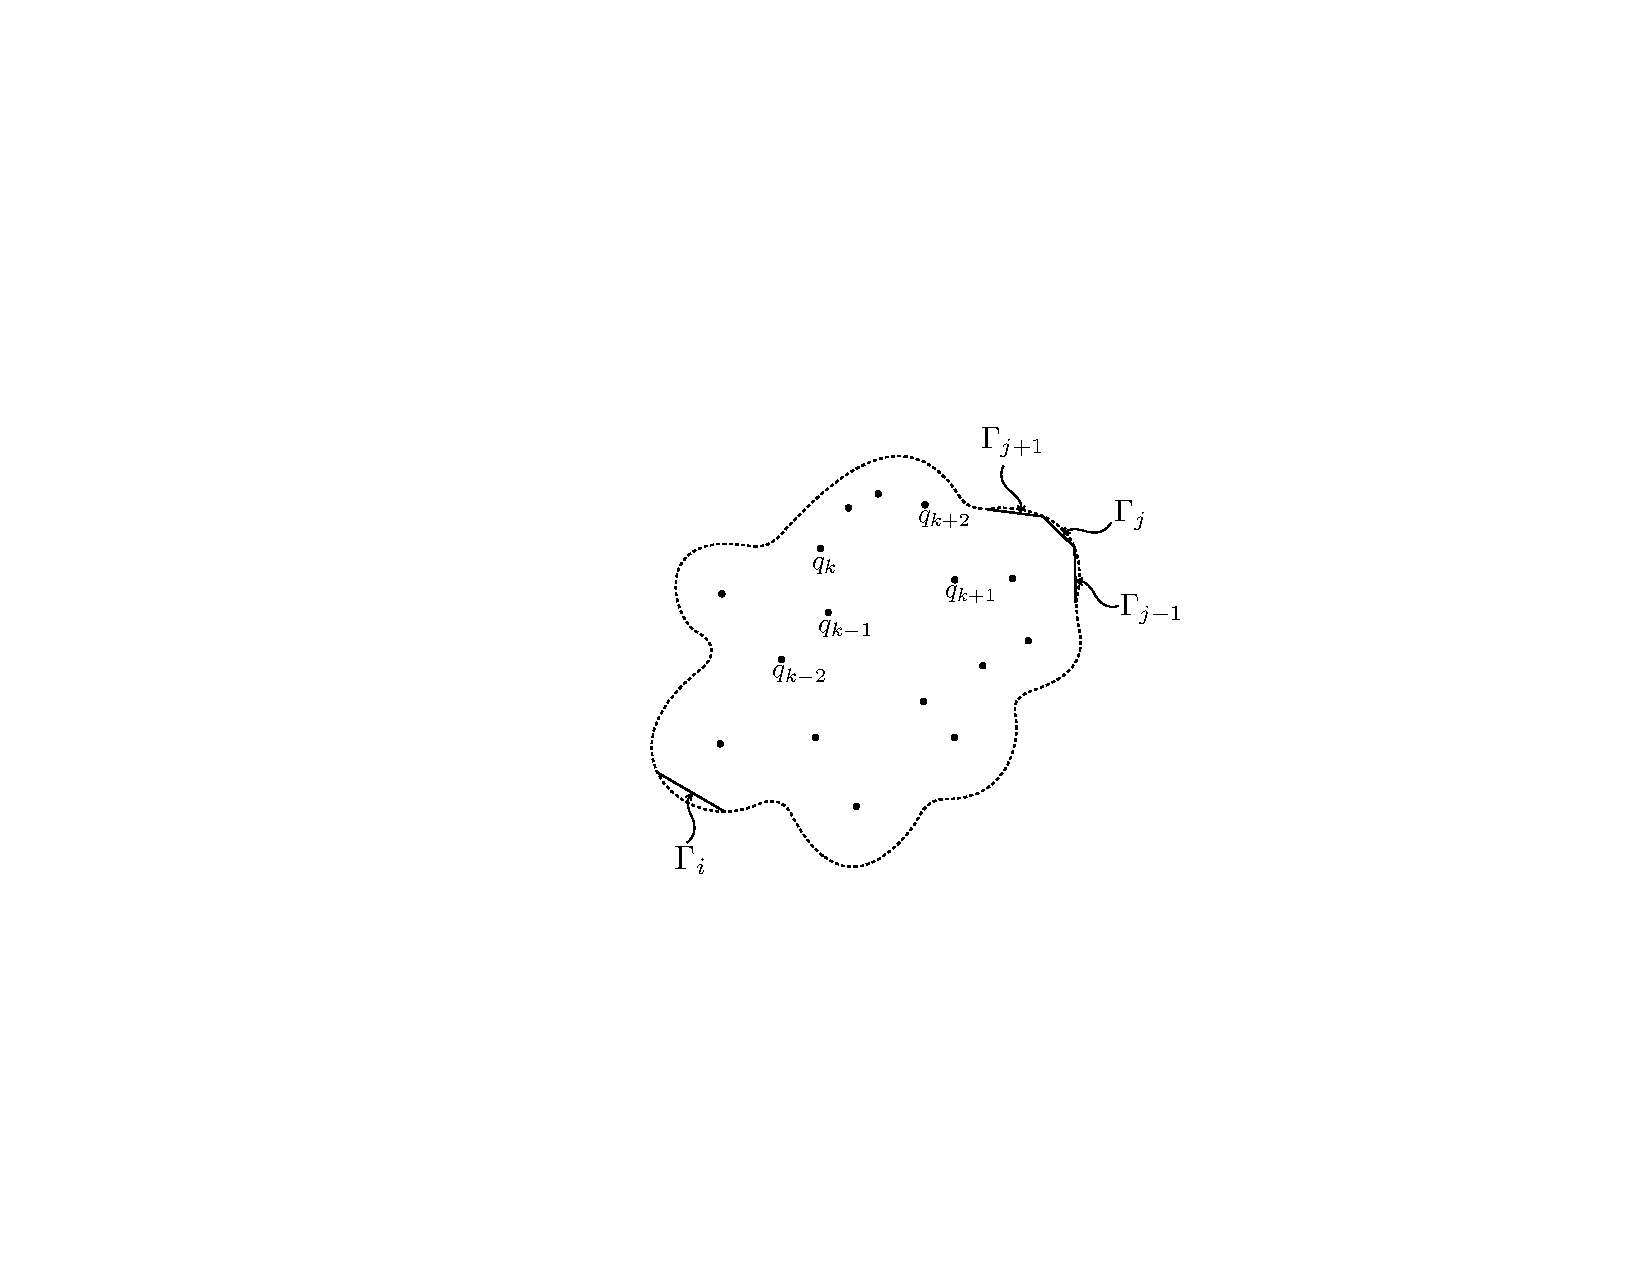
\includegraphics[width=0.25\textwidth]{Figure3.pdf}
   \caption{Structure of protein \gb (\pdb code {\small 1PGB}).}
   \label{fig:1pgb}
\end{figure}

\begin{figure}%[h] 
   \centering
   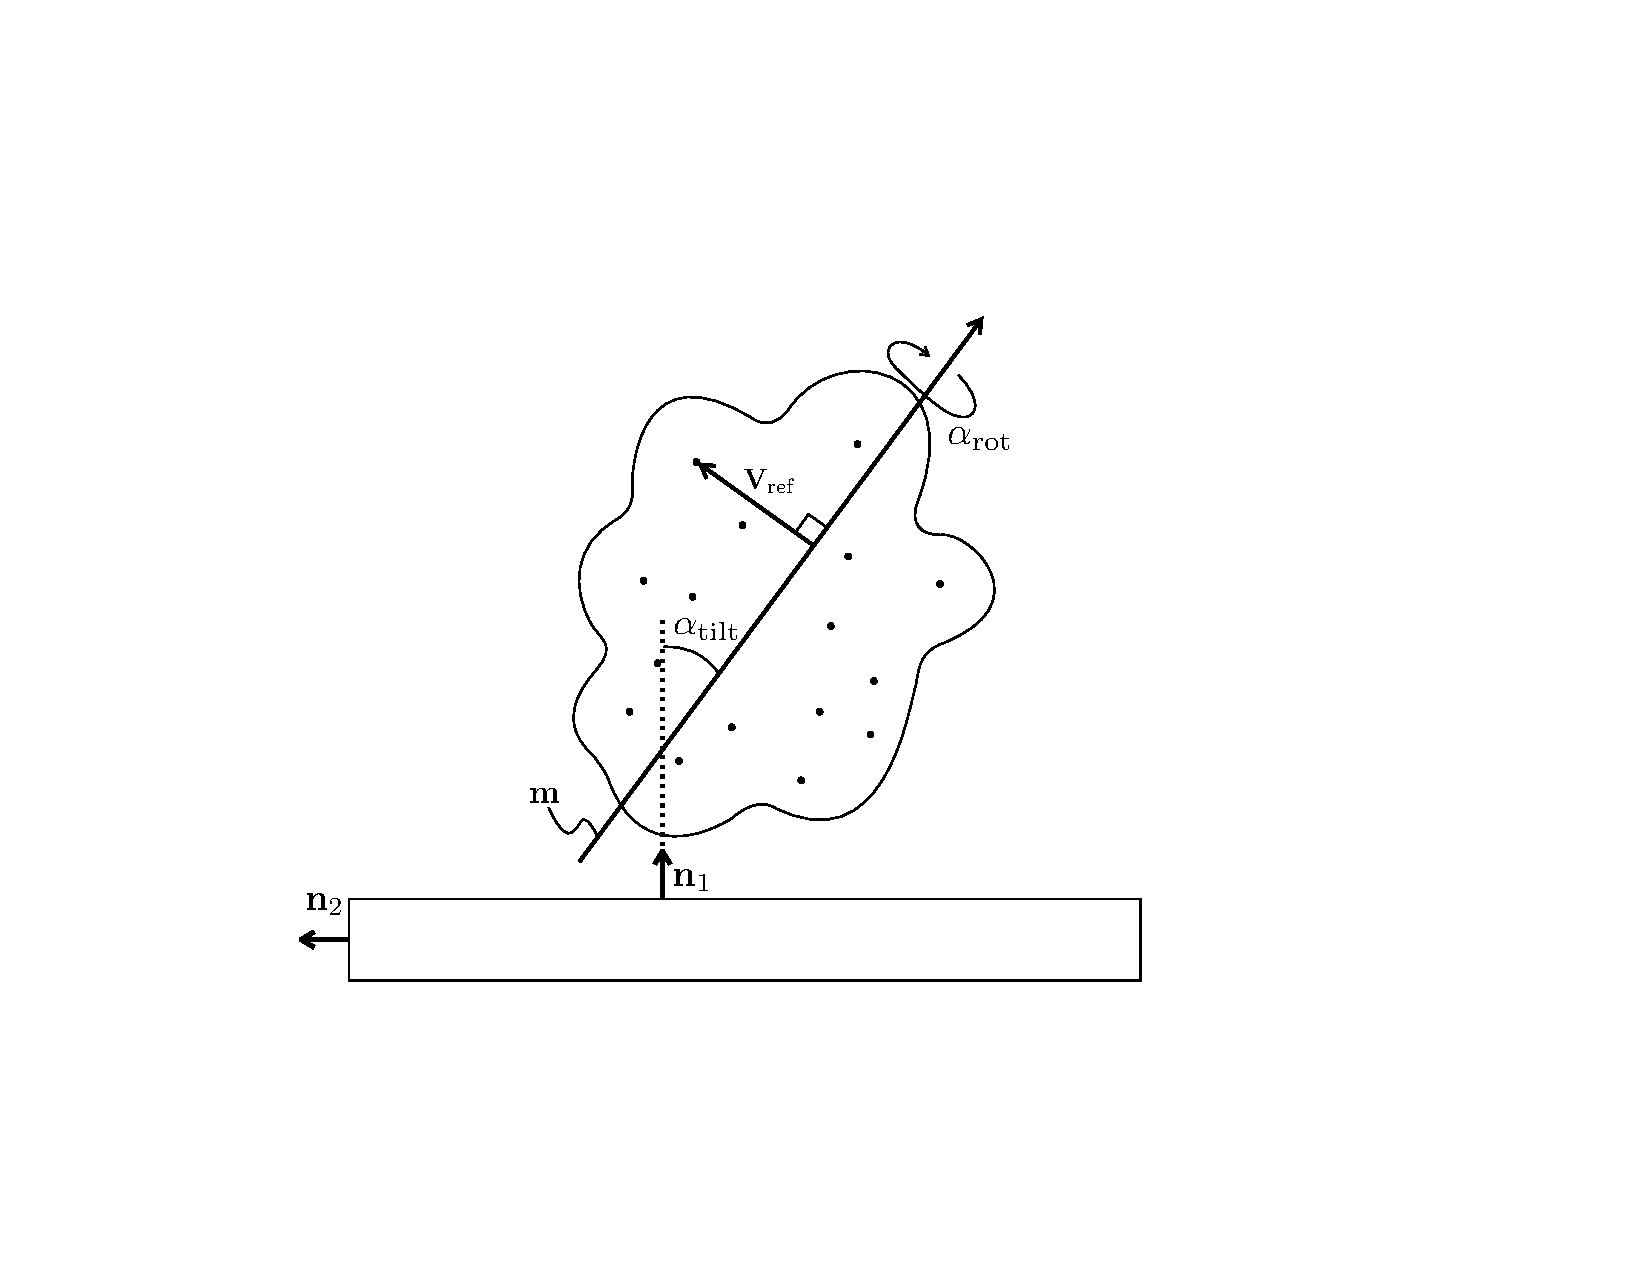
\includegraphics[width=0.35\textwidth]{Figure4.pdf}
   \caption{Structure of immunoglobulin G (\pdb code {\small 1IGT}).}
   \label{fig:1igt}
\end{figure}

